\chapter{Feed forward networks}

\section{Perceptron}

The building block of a neural network is the \textbf{perceptron\index{perceptron}} which is a mathematical model of a biological neuron, or brain cell. Similar to how neurons have dendrids, a perceptron has inputs and an \textbf{activation function\index{activation function}}. The inputs are fed in as a linear combination, with each input being assigned a weight. Weights are usually real numbers.


\begin{figure}[htbp]
    \begin{center}
        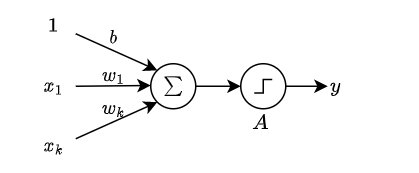
\includegraphics[width=150pt]{../img/07-perceptron.png}
        \caption{Figure 7.1: Model of a neuron}
    \end{center}
\end{figure}


We can model the combination of inputs and weights as a dot product. The threshold of activation or \textbf{bias\index{bias}} of the perceptron is modelled with an added input \(1\) and a weight noted with \(b\). The dot product becomes \(z = b + w \cdot x = b + \sum_j w_jx_j\).

For the neural network to be able to approximate any function, needs to non linear. Since inputss and weights are linear combination, this non liniarity is achieved trough the activation function which in most cases is not linear.

Neural networks use various functions as activation functions:


\begin{figure}[htbp]
    \begin{center}
        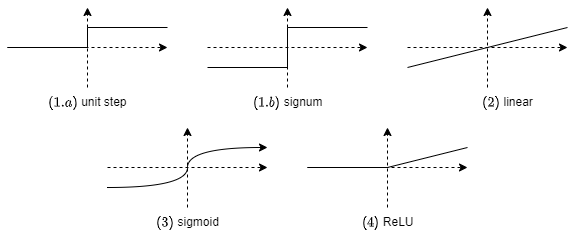
\includegraphics[width=300pt]{../img/07-activation-functions.png}
        \caption{Figure 7.4: Activation functions}
    \end{center}
\end{figure}


\begin{enumerate}
    \item \textbf{Step function\index{Step function}}: can be either unit step

\[h = \begin{cases}
0 & \operatorname{if }\ z > 0 \\
1 & \operatorname{if }\ z \le 0
\end{cases}
\]

or signum, where \(-1\) is used instead of \(0\). The challenge with this is that small change in the input might trigger a jump from \(0\) to \(1\) times weights, which might be a sudden big jump and if organized to network it might not learn.

    \item \textbf{Linear\index{Linear}}

\[h = z \]

Same as linear regression. In case multiple neurons are connected will still collapse to linear model. To be able to model non linear functions, the activation should also be non linear

    \item \textbf{Sigmoid\index{Sigmoid}}

\[h = {1 \over 1 + e^{-z}}\]

Small changes in the input will result in small changes in the output because the function is continuous.

\[\Delta h \approx \sum_j {\partial h \over \partial w_j} \Delta w_j \]

Sigmoid can become saturated on values close to \(0\) (low) and \(1\) (high) because the derivate becomes close to \(0\).

    \item \textbf{Rectifier Linear Unit: ReLU\index{Rectifier Linear Unit: ReLU}}

\[h = max(0, z)\]

A variant is the \textbf{leaky ReLU\index{leaky ReLU}} which allows small negative values to be passed trough. It:s defined as

\[h = max(az, z)\]

where \(a\) is a very small constant (e.g. \(0.0001\)). While the rectified unit is not continuous and it has some issues like vanishing or exploding gradient in learning, it's still very popular due to it's simplicity and good performance in practice if used as part of large neural networks.
\end{enumerate}

\section{Network structure}

In feed forward networks, output of neurons in a layer act as inputs in the next layer


\begin{figure}[htbp]
    \begin{center}
        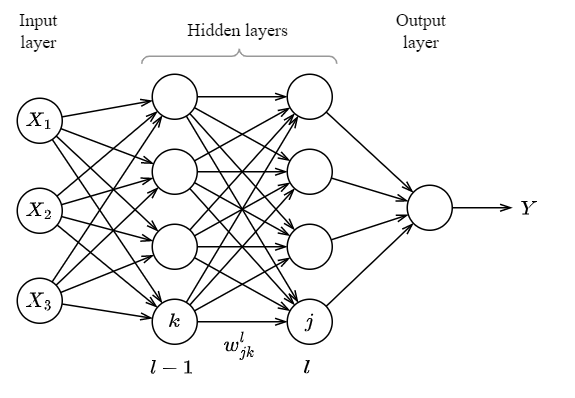
\includegraphics[width=287pt]{../img/07-feedforward-network.png}
        \caption{Figure 7.3: Architecture of a feed forward neural network with 3 inputs and 2 hidden layers}
    \end{center}
\end{figure}


To train the model we can choose a loss function \(C\) we could minimize. To minimize \(C\) we can define a change in \(C\) as the sum of all partial derivates of \(C\) over all the weights \(w_k\)

\begin{equation}\Delta C \approx \sum_k { \partial C \over \partial w_k} \Delta w_k = \nabla C \Delta w_k \tag{7.1}\end{equation}

\(\nabla C\) (pronounced nabla) is simply a notation for the sum of partial derivates. We can make a decrease in the cost function \(C\) by choosing \(\Delta w_k\) as

\[\Delta w_k = -\eta \nabla C\]

Where \(\eta\) is the learning rate. Plugging it to (7.1) we get

\[\Delta C \approx - \eta \| \nabla C \| ^ 2\]

Since \(\| \nabla C \| ^ 2\) is positive, \(- \eta\) is negative, so will always result in moving in direction of decrease in \(\Delta C\). The update rule of weights to minimize the cost function \(C\) is

\begin{equation}w_k' = w_k - \eta { \partial C \over \partial w_k}\tag{7.2}\end{equation}

Similarly we can write the same for bias as well

\begin{equation}b' = b - \eta { \partial C \over \partial b}\tag{7.3}\end{equation}

\subsection{Cost functions}

The MSE seen in Chapter 3 is often used with ReLU but does not work well with sigmoid neurons or if the output layer is a softmax layer (see below).

If the neuron is saturated on the opposite value which it has to learn, adjusting from one side to another will require many learning iterations, the initial learning rate being very slow (until the learning gets to the steep part of the sigmoid function). Because of this limitation, a better alternative to be used with sigmoid is the \textbf{cross entropy cost function\index{cross entropy cost function}}

\begin{equation}C = -{1 \over n}\sum_x[y \ln a + (1 - y) \ln (1-a)] \tag{7.5}\end{equation}

Cross entropy definition relates to entropy in information theory (see \#todo under trees): cross entropy measures the \textit{s}urprise\textit{ }when we learn the true probability \(y\) for a predicted probability \(a\) as \(H(y,a) = -\sum_xy_i\log_2(a_i)\), using natural log \(\ln\) instead of \(\log\), which is same from optimization perspective (ratio is a constant of \(\ln 2\)). (7.5) is a special case of cross entropy also called \textbf{binary cross entropy\index{binary cross entropy}} (we will refer to it simply as cross entropy cost function), which has two terms to penalize prediction of true label if actual label is false and also penalize prediction of false label when actual label is true.

Cross entropy cost function acts as a cost function because it's always positive (both terms in the sum are negative for \(a \in [0, 1]\) making overall result positive) and for small differences between \(y\) and \(a\), will result in a small result as cost.

To see why this seemingly complex function is useful, we could check the learning rate for a single sigmoid neuron, notated with \(\sigma(z)\) the partial derivate against a weight \(w\):

\({\partial C \over \partial w_j} = {\partial \over \partial w_j }{\big ( -{1 \over n}\sum_x(y \ln \sigma(z) + (1 - y) \ln (1-\sigma(z)))\big ) }\)

\(= -{1 \over n}\sum_x \left ( {\partial \over \partial w_j}\big ( y \ln \sigma(z)\big ) + {\partial \over \partial w_j} \big ((1 - y) \ln (1-\sigma(z))\big )\right )\)

Because \(ln(x)' = {1 \over x}\)

\({\partial C \over \partial w_j} = -{1 \over n}\sum_x \left ( {y \over \sigma(z) } {\partial \sigma(z) \over \partial w_j} - {1 - y \over 1-\sigma(z)} {\partial \sigma(z) \over \partial w_j}\right )\)

Notice how the sign in the middle flipped because of \(ln'(1-\sigma(z))\)

\({\partial C \over \partial w_j} = -{1 \over n}\sum_x \left ( {y \over \sigma(z) } - {1 - y \over 1-\sigma(z)}\right ) {\partial \sigma(z) \over \partial w_j} \)

Since \(z = b + \sum_j x_jw_j\) the derivate will be \({\partial \sigma(z) \over \partial w_j} = \sigma'(z) z'(w_j) = \sigma'(z) x_j\), pluggin in

\({\partial C \over \partial w_j} = -{1 \over n}\sum_x \left ( {y \over \sigma(z) } - {1 - y \over 1-\sigma(z)}\right ) \sigma'(z)x_j\)

We can rewrite \({y \over \sigma(z) } - {1 - y \over 1-\sigma(z)} = {y(1-\sigma(z)) - (1 - y)\sigma(z) \over \sigma(z) (1-\sigma(z)) } = {y - \sigma(z) - y\sigma(z) + y\sigma(z) \over \sigma(z) (1-\sigma(z))} = {y - \sigma(z) \over \sigma(z) (1-\sigma(z))}\). We get

\({\partial C \over \partial w_j} = -{1 \over n}\sum_x \left ( {y - \sigma(z) \over \sigma(z) (1-\sigma(z))}\right ) \sigma'(z)x_j\)

Using the definition of sigmoid \(\sigma(z) = {1 \over 1 + e^{-z}}\), and the rule \(\left( 1 \over f \right )' = (f^{-1})' = -f^{-2} f'\) we can calculate\\

\(\sigma'(z) = \left (-{1 \over ( 1 + e^{-z})^2} \right ) e^{-z} (-1)\) \\
\(= {e^{-z} \over ( 1 + e^{-z})^2 } = {1 \over  1 + e^{-z}} {e^{-z} \over 1 + e^{-z}} = {1 \over  1 + e^{-z}} {1 + e^{-z} - 1 \over 1 + e^{-z}} = {1 \over 1 + e^{-z}} \left ( 1 - {1 \over  1 + e^{-z}} \right ) \)\\
\(= \sigma(z)(1 - \sigma(z))\). \\
Plugging the result, i.e \(\sigma'(z) = \sigma(z)(1 - \sigma(z))\) to \({\partial C \over \partial w_j}\) will give

\({\partial C \over \partial w_j} = -{1 \over n}\sum_x \left ( {y - \sigma(z) \over \sigma(z) (1-\sigma(z))}\right ) \sigma(z)(1 - \sigma(z)) x_j \)\\
\(= -{1 \over n}\sum_x(y - \sigma(z))x_j\)

\[{\partial C \over \partial w_j} = {1 \over n}\sum_x(\sigma(z) - y)x_j\]

The result shows that the learning rate \({\partial C \over \partial w_j}\) is proportional to the difference between expected and actual output \(y - \sigma(z)\). The larger the difference the better the learning rate. The same is not true if we use MSE with sigmoid.

We can claculate the same for bias the only difference is \({\partial \sigma(z) \over \partial b} = \sigma'(z) z'(b) = \sigma'(z)\), resulting in

\[{\partial C \over \partial b} = {1 \over n}\sum_x(\sigma(z) - y)\]

Cross entropy giving a simple result when calculating gradients makes it a good choice to improve the learning rate.

Less popular but the negative log likelyhood function might also be used with softmax output.

\section{How networks learn}

Training neural networks can be highly inefficient so we need various optimizations. First we optimize on how we use the input data. To calculate the rate of change in cost function (7.4) or (7.5) we could iterates trough all input data, but this process would be costly. Instead of calculating the change in cost function for all inputs, we can select a subset of size \(m\) of training data, noted with \(X_j\), called \textbf{mini batch\index{mini batch}} to update the weights. The update would take the form

\[w_k' = w_k - {\eta \over m} { \partial C_{X_j} \over \partial w_k} \]

In some cases the \(1 \over m\), which scales the learning rate with batch size, can be ommitted. A complete iteration over all training data trough batches is called an \textbf{epoch\index{epoch}}.

Trough the example of cross entropy, we looked at how a single neuron learns but calculating the same way how an entire network learns is not efficient. All forward paths would need to be distangled and summed up several times. It would basically mean recalculating every subtree every time it shows up after a perceptron as we step trough the graph. Instead more efficient algorithms can be used which move backward, reusing already computed results.

\textbf{Backprograpagation\index{Backprograpagation}} is the algorithm used in training, specifically for calculating \(\partial C \over \partial w\)  and \(\partial C \over \partial b\) from equations (7.2) and (7.3) respectively for a multi layer neural network.

\subsection{Assumptions of backpropagatation}

\begin{enumerate}
    \item The cost function \(C\) can be written as the average of the cost function for all training samples \(x\) noted \(C_x\). This assumption is needed because backpropagation is done per training sample
\end{enumerate}

\[C = {1 \over n} C_x\]

\begin{enumerate}
    \item The cost function can be written as a function of the outputs of the network. Having \(L\) as the number of layers
\end{enumerate}

\[C = C(A^L)\]

\textbf{Notations\index{Notations}}

\begin{itemize}
    \item \(w_{jk}^l\) as the weight from \(k\) th neuron in \(l-1\) th layer to \(j\) neuron in \(l\) th layer (figure 7.5)
    \item \(b_j^l\) is bias of the \(j\) th neuron in layer \(l\)
    \item \(h\) activation method used
    \item \(A_j^l\) is activation of the \(j\) th neuron in layer \(l\)
\end{itemize}

   The activation function

   \[A_j^l = h(b_j^l + \sum_k w_{jk}^l A_j^{l-1})\]

Transforming to matrix form

\begin{itemize}
    \item \(w^l\) is the weight matrix of layer \(l\) where columns are  \(k\) (\(l-1\) layer neuron) and rown are \(j\) (\(l\) layer neuron) for weight \(w_{jk}^l\)
    \item \(b^l\) bias vector
    \item Applying a function to a vector is equivalent of applying to all vector elements: \(h(z)_j \equiv h(z_j)\)
    \item \(A^l\) activation vector becomes\[A^l = h(z^l) = h(b^l + w^l A^{l-1})\] The reversal of order of \(j\) and \(k\) in \(w_{jk}^l\) is to eliminate the transpose \(w^T\) of weight matrix \(w\) in the above equation.
    \item Hadaman product is the element wise product of two vectors resulting in a vector, noted with \(\odot\) \[(s \odot t)_j = s_j t_j\]
\end{itemize}


\subsection{ Equations of backpropagation}

Backpropagation is an algorithm to calculate \({\partial C \over \partial w^l}\) and \({\partial C \over \partial b^l}\), by introducing an error term in the \(j\) th neuron noted with \(\delta_j^l\)

By making a weighted input change of a neuron \(\Delta z_j^l\), this would cause the output of neuron to be \(h(z_j^l + \Delta z_j^l)\), overall cost would change \({\partial C \over \partial z_j^l} \Delta z_j^l\). To minimize cost, we can choose \(\Delta z_j^l\) to be \(- {\partial C \over \partial z_j^l}\), so that it would result in a minus squared term which is always negative, and thus would help us reduce the cost function. Thus the error term we can choose is

\begin{equation}\delta_j^l = {\partial C \over \partial z_j^l} \tag{7.6}\end{equation}

The vector \(e^l\) is the error term for layer \(l\).

\textbf{Error in out payer\index{Error in out payer}} (element wise and matrix form):

\[\delta_j^L = {\partial C \over \partial A_j ^ L} h ' (z_j^L)\]

\begin{equation}\delta^L = \nabla _AC \odot h(z^L) \tag{BP1}\end{equation}

Proof:

\begin{flalign*}
& \text{Start with (7.6)} \\
& \delta_j^l = {\partial C \over \partial z_j^l} \\
& \text{applying the chain rule} \\
& \delta_j^l = \sum_k{\partial C \over \partial A^L_k}{\partial A^L_k \over \partial z_j^l} \\
& \text{Since activation} A \text{of} k \text{th neuron depends only of the weighted input of the same neuron} z \text{we can eliminate all terms where} k \ne j \\
& \delta_j^l = {\partial C \over \partial A^L_j}{\partial A^L_j \over \partial z_j^l} \\
& \text{Because by definition} A^L_j = h(z_j^L) \text{we can rewrite the second term} \\
& \delta_j^l = {\partial C \over \partial A^L_j}h'(z_j^L) \\
&  \\ && \end{flalign*}

\textit{*}Error of layer \(l\) in respect to error in laer \(l+1\)\textit{*}

\begin{equation}\delta^l = \big ((w^{l+1})^T \delta^{l+1}\big ) \odot h(z^l) \tag{BP2}\end{equation}

The first half moves the error backward a layer, the second half, moves error trough the layer

(BP1) and (BP2) allow calculating the error \(e\) for all layers

Proof:

\begin{flalign*}
& \text{Start with (7.6)} \\
& \delta_j^l = {\partial C \over \partial z_j^l} \\
& \text{applying the chain rule, in terms of} \\
& \delta_j^{l+1} = {\partial C \over \partial z_j^{l+1}} \\
& \text{we get} \\
& \delta_j^l = \sum_k{\partial C \over \partial z_j^{l+1}}{\partial z_j^{l+1} \over \partial z_j^l} \\
& \delta_j^l = \sum_k{\partial z_j^{l+1} \over \partial z_j^l}\delta_k^{l+1} \\
& \text{The first term} \\
& {\partial z_j^{l+1} \over \partial z_j^l} = {\partial \sum_j w_{kj}^{l+1} f(z_j^l) + b_k^{l+1} \over \partial z_j^l} = w_{kj}^{l+1}h'(z_j^l) \\
& \text{Adding it back} \\
& \delta_j^l = \sum_k w_{kj}^{l+1} \delta_k^{l+1} h'(z_j^l) \\
& \text{Writing the same in matrix form we get} \\
& \delta^l = \big ((w^{l+1})^T \delta^{l+1}\big ) \odot h(z^l) \\ && \end{flalign*}

\textbf{Rate of change of cost in respect to bias\index{Rate of change of cost in respect to bias}}

\begin{equation}{\partial C \over \partial b^l} = \delta^l \tag{BP3}\end{equation}

Proof:

\begin{flalign*}
& {\partial C \over \partial b^l} = \sum_k {\partial C \over \partial z_k^l}{\partial z_k^l \over \partial b_j^l} \\
& \text{Since} z_k^l \text{only dependson on} b_j^l \text{where} k = j \\
& {\partial C \over \partial b^l} = {\partial C \over \partial z_j^l}{\partial z_j^l \over \partial b_j^l} = \delta^l{\partial z_j^l \over \partial b_j^l} \\
& {\partial C \over \partial b^l} = \delta^l{\partial \sum_j w_{kj}^l f(z_j^{l-1}) + b_k^l \over \partial b_j^l} \\
& \text{The second term is simply} 1 \text{resulting in} \\
& {\partial C \over \partial b^l} = \delta^l \\ && \end{flalign*}

\textbf{Rate of change of cost in respect to weights\index{Rate of change of cost in respect to weights}}

\begin{equation}{\partial C \over \partial w^l} = A^{l-1}\delta^l \tag{BP4}\end{equation}

Proof

\({\partial C \over \partial w^l} = \sum_m {\partial C \over \partial z_m^l}{\partial z_m^l \over \partial w_{kj}^l}\)

\({\partial C \over \partial w^l} = \sum_m {\partial C \over \partial z_m^l}{\partial \sum_n w_{mn}^lA_n^{l-1} + b_m^l \over \partial w_{kj}^l}\)

and only when \(m = j\) and \(n = k\), the derivative is not \(0\), so here we get

\({\partial C \over \partial w_{jk}^l} = {\partial C \over \partial z_j^l}A_k^{l-1} = A^{l-1}\delta^l\)

\subsection{Algorithm of backpropagation}

The algorithm (using mini batches)

\begin{enumerate}
    \item For each input of a mini batch \(x\), use as \(A^1\) of input layer
            \begin{enumerate}
            \item Feed forward trough layers \(l = 2, 3, ..., +L\) with \(z^l = w^lA^{l-1} + b^l\) and \({A^l} = h(z^l)\)
            \item Calculate output error with (BP1)
            \item Backpropagate error with (BP2)
        \end{enumerate}
    \item Adjust weights and biases with learning rate times the average of gradients given by (BP3) and (BP4)
\end{enumerate}

The reason backpropagation is faster than forward learning is because we would need to compute the gradient for all combinations of weights for each layer. Since most of the computation is redundant in the sense that partial gradients are recalculated multiple times, for each forward path, the backpropagation algoroithm optimizes on this to compute only once.

\section{Techniques used to improve learning}

In recent years a number of techniques has been developed to improve the performance of neural networks

\subsection{Softmax output layer}

Softmax can be used with both ReLU and sigmoid activation functions, but works best with the cross entropy cost function. The softmax is similar to a multi variate logistic regression. We apply it to the last layer of the network only, noted with \(L\)

\[A_j^L = {e^{z_j^L} \over \sum_k e^{z_k^L}}\]

The output of softmax normalizes all outcomes to always sum up to \(1\).

\[\sum_k A_k^L = {\sum_k e^{z_k^L} \over \sum_k e^{z_k^L}} = 1\]

The output is always positive since \(e^x\) is always positive. These two propoerties make the softmax function a probability distribution, which means we can treat the output of a network as an estimated probibility for each classification.

\section{References}

\textbf{An Introduction to Statistical Learning, with applications in R, Second Edition\index{An Introduction to Statistical Learning, with applications in R, Second Edition}}, Gareth James, Daniela Witten, Trevor Hastie, Rob Tibshirani

\textbf{Neural Networks and Deep Learning\index{Neural Networks and Deep Learning}}, Michael Nielsen 2019

